\documentclass[]{article}
\usepackage{graphicx}

%opening
\title{Parallellisme - Project report}
\author{Hans Van der Ougstraete}

\begin{document}

\maketitle
\clearpage
\tableofcontents
\clearpage

\section{Implementatie}

\subsection{Fase 1}
Fase 1 is opgedeeld in twee delen, het eerste deel maakt een lijst met relevante businesses door in de base case de evaluaterevalence methode uit SequentialSearch aan te roepen. De Yelpdata wordt dus in stukken opgedeeld tot het kleinste deel een business is. Deze lijst wordt in het tweede deel aan de hand van een parallele mergesort gesorteerd. Deze code is terug te vinden in de ParallelSearch klasse.
\subsection{Fase 2}
In progress
\section{Evaluatie}
De benchmarks op eigen computer (quad core i5-2300 @2.80GHz) zijn 4 maal uitgevoerd. Voor SequentialSearch, ParallelSearch met 1, 2 workers en ParallelSearch met 4 workers. Dit telkens 1500 keer. De resultaten worden per preset weergegeven.

\subsection{Fase 1}

\begin{table}[h!]
	\centering
\begin{tabular}{|c|c|c|c|}
	\hline 
	Runtime ms & Preset1 & Preset2 & Preset3 \\ 
	\hline 
	Parallel P=1 & 466 & 514 & 145 \\ 
	\hline 
	Parallel P=2 & 304 & 328 & 111 \\ 
	\hline 
	Parallel P=4 & 273 & 291 & 108 \\ 
	\hline 
	Sequential & 451 & 381 & 134 \\ 
	\hline 
\end{tabular}
\caption{Gemiddele runtime in miliseconden}
\label{table:1}
\end{table}

\begin{figure}
	\centering
	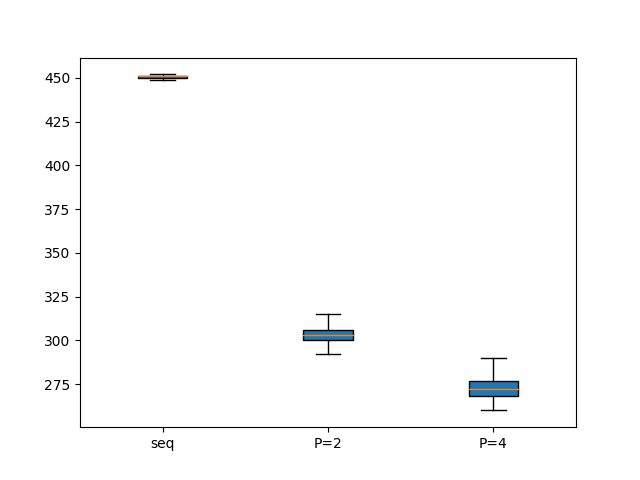
\includegraphics[width=0.7\linewidth]{Preset_1}
	\caption[Preset1]{Preset1}
	\label{fig:preset1}
\end{figure}

\begin{figure}
	\centering
	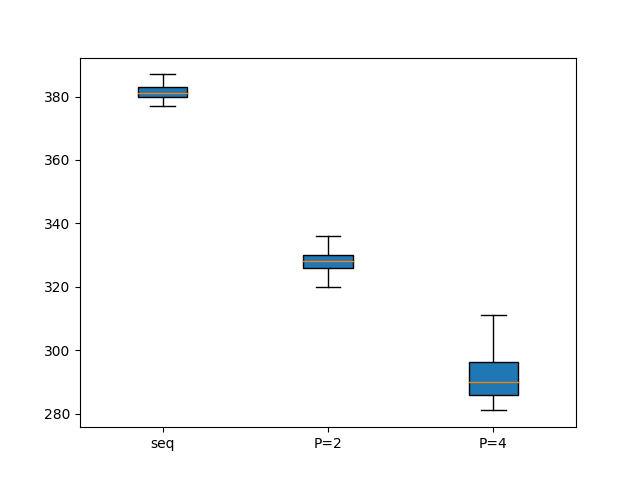
\includegraphics[width=0.7\linewidth]{Preset_2}
	\caption[Preset1]{Preset2}
	\label{fig:preset2}
\end{figure}

\begin{figure}
	\centering
	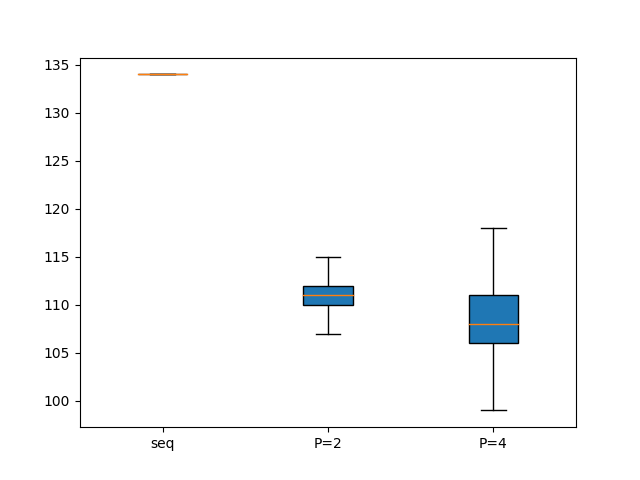
\includegraphics[width=0.7\linewidth]{Preset_3}
	\caption[Preset1]{Preset3}
	\label{fig:preset3}
\end{figure}

\subsubsection{Overhead}

\begin{table}[h!]
	\centering
\begin{tabular}{|c|c|c|c|}
	\hline 
	Overhead & Preset1 & Preset2 & Preset3 \\ 
	\hline 
	T1/Tseq & 1.03 & 1.35 & 1.08 \\ 
	\hline 
\end{tabular} 
\caption{Overhead waarden voor de 3 presets.}
\label{table:2}
\end{table}

Bovenstaande tabel toont de overhead, deze overhead van het verdelen in threads is niet aanwezig bij de sequentiële versie omdat de sequentiële versie niet opdeelt in alsmaar kleinere taken. De overhead is verschillend per preset omdat het opdelen van het werk afhangt van de respectievelijke data.
De overhead kan kleiner gemaakt worden door een goede cut-off waarde te gebruiken, hierdoor wordt er sneller sequentieel gewerkt en daardoor minder opgedeeld in subtaken.

\subsubsection{Speed-up}
\begin{table}[h!]
	\centering
	\begin{tabular}{|c|c|c|c|}
		\hline 
		Speed-up & Preset1 & Preset2 & Preset3 \\ 
		\hline 
		Tseq/T2 & 1.48 & 1.16 & 1.21 \\ 
		\hline 
		\hline 
		Tseq/T4 & 1.65 & 1.31 & 1.24 \\ 
		\hline 
	\end{tabular} 
	\caption{Speed-up values for all 3 presets.}
	\label{table:2}
\end{table}

Een perfecte speed-up zou gelijk zijn aan het aantal extra processors, dit is hier niet het geval.
De speed-up is ook verschillend per preset, het aantal businesses en revieuws beïnvloeden dit volgens mij.
Bij preset 3 is er nauwelijks verschil tussen T=2 en T=4, ik veronderstel dat dit is omdat de data klein is.
het meeste winst wordt geboekt bij preset 1, de preset met het meest aantal businesses.

\subsection{Fase 2}

Het doorzoeken van de revieuw om het aantal voorkomens van een woord te bepalen kan op verschillende manieren.
Er bestaat een java klasse split welke een text opdeelt en per woord in een vector stopt. Echter had ik wat moeilijkheden om de reguliere expressie die aangeeft waar een woord eindigt (bv spatie of leesteken) zo in te stellen dat de unit tests slagen. Ik had net iets meer of minder voorkomens dan de sequentiële search. Zonder controle over de input van de revieuws zou een reguliere expressie die voor een preset werkt misschien in een andere preset iets over het hoofd kijken. Een ander mischien betere oplossing is het gebruik van hashmaps, hierbij wordt het voorkomen van ieder woord geteld. Deze hash opslagen zou bij een volgende zoektocht snel het aantal voorkomens uit de hash kunnen halen. In deze hash zijn de woorden de key's en het aantal voorkomens de value.



\end{document}
